\documentclass[12pt,a4paper]{article}

\usepackage{fontawesome5}
\providecommand{\faPencilAlt}{\faIcon{pencil-alt}}

\usepackage{styles/couleurs}
\usepackage{styles/mise_en_page}
\usepackage{styles/boites}
\usepackage{styles/maths}
\usepackage{styles/figures}

\usepackage{enumitem}
\usepackage{array}
\usepackage{tabularx}
\usepackage{amsmath}
\usepackage{amssymb}
\usepackage{tikz}
\usepackage{xparse}
\usepackage{pdflscape}
\usepackage{colortbl}

\usetikzlibrary{calc,arrows.meta,positioning}

\setlist[itemize]{leftmargin=1.4em,itemsep=0.15em,topsep=0.2em}
\setlist[enumerate]{leftmargin=*,itemsep=0.22em,topsep=0.25em}

\newcommand{\lignepointillee}{\noindent\dotfill\par\vspace{0.45em}}

\newcommand{\lignesreponse}[1]{%
\begin{tcolorbox}[
enhanced,colback=white,colframe=NeutreC!40,boxrule=0.5pt,arc=1.5mm,
left=3mm,right=3mm,top=2mm,bottom=1mm,before skip=2pt,after skip=2pt]
\foreach \i in {1,...,#1}{\lignepointillee}
\end{tcolorbox}}

\newcommand{\titreseq}[1]{%
\begin{center}
{\sffamily\LARGE\bfseries\color{TitreC}Séquence 7 -- Arithmétique}\\[0.2em]
{\sffamily\large\bfseries\color{SavoirC}#1}
\end{center}}

\newcommand{\grillecent}{%
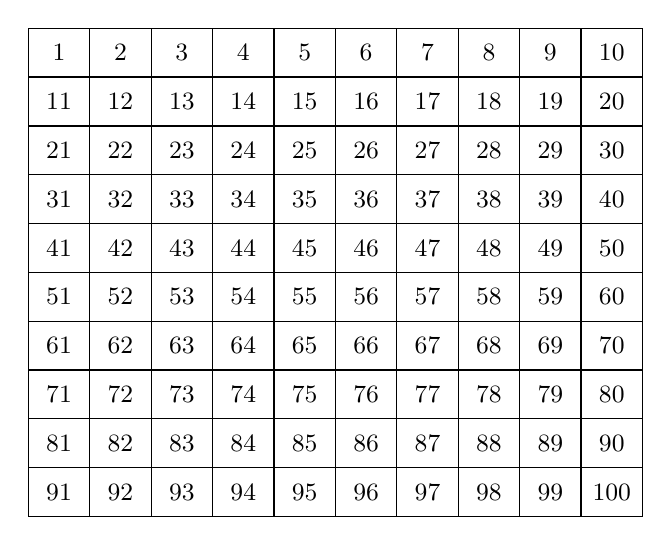
\begin{tikzpicture}[x=0.78cm,y=0.62cm]
  \foreach \n in {1,...,100}{
    \pgfmathtruncatemacro{\col}{mod(\n-1,10)}
    \pgfmathtruncatemacro{\lig}{9-floor((\n-1)/10)}
    \draw[line width=0.45pt] (\col,\lig) rectangle ++(1,1);
    \node[font=\small] at (\col+0.5,\lig+0.5) {\n};
  }
\end{tikzpicture}}

\begin{document}

\titreseq{Automatismes -- Séries courtes}

\remarque{Chaque série est prévue pour environ cinq minutes.
La justification demandée tient généralement en une phrase ou une égalité.}

\section*{Série 1 -- Multiple ou diviseur ?}

Complète avec « multiple » ou « diviseur ».

\begin{enumerate}
  \item \(7\) est un \dotfill{} de \(42\).
  \item \(60\) est un \dotfill{} de \(12\).
  \item \(5\) est un \dotfill{} de \(35\).
  \item \(81\) est un \dotfill{} de \(9\).
\end{enumerate}

\section*{Série 2 -- Division euclidienne}

Complète :

\[
157=12\times\ldots+\ldots
\]

\[
304=25\times\ldots+\ldots
\]

Le reste doit toujours vérifier : \(\dotfill\).

\section*{Série 3 -- Critères de divisibilité}

Sans poser de division, indique si \(4\,590\) est divisible par :

\[
2\qquad 3\qquad 5\qquad 9\qquad 10.
\]

Justifie chaque réponse par un critère.

\section*{Série 4 -- Lister}

\begin{enumerate}
  \item Donne les six premiers multiples de \(7\).
  \item Donne tous les diviseurs de \(24\).
  \item Donne trois multiples communs à \(4\) et \(6\).
\end{enumerate}

\section*{Série 5 -- Premier ou composé ?}

Indique si chaque entier est premier.
S'il ne l'est pas, donne un diviseur non trivial.

\[
29\qquad 39\qquad 47\qquad 51\qquad 73\qquad 91.
\]

\section*{Série 6 -- Liste des nombres premiers}

Complète les nombres premiers manquants :

\[
2,\ 3,\ 5,\ 7,\ 11,\ \ldots,\ 17,\ 19,\ \ldots,\ 29.
\]

\[
31,\ 37,\ \ldots,\ 43,\ 47,\ \ldots.
\]

\section*{Série 7 -- Décomposer}

Décompose en produit de facteurs premiers :

\[
36\qquad 45\qquad 70\qquad 84.
\]

\section*{Série 8 -- Vérifier une décomposition}

Pour chaque égalité, indique si elle est correcte.

\[
90=2\times3\times3\times5
\]

\[
126=2\times3\times7\times3
\]

\[
75=3\times5\times5
\]

\[
44=2\times2\times11.
\]

\section*{Série 9 -- Simplifier une fraction}

Simplifie en utilisant les facteurs premiers :

\[
\frac{18}{30}
\qquad
\frac{42}{63}
\qquad
\frac{70}{105}.
\]

\section*{Série 10 -- Fractions égales}

Parmi les fractions suivantes, lesquelles sont égales ?

\[
\frac{6}{15}
\qquad
\frac{10}{25}
\qquad
\frac{14}{35}
\qquad
\frac{15}{36}.
\]

\section*{Série 11 -- Groupes identiques}

On veut répartir \(36\) objets rouges et \(48\) objets bleus
dans des groupes identiques sans reste.

\begin{enumerate}
  \item Peut-on faire \(6\) groupes ?
  \item Peut-on faire \(8\) groupes ?
  \item Donne deux autres nombres de groupes possibles.
\end{enumerate}

\section*{Série 12 -- Vrai ou faux ?}

Justifie en une ligne.

\begin{enumerate}
  \item Tous les nombres premiers sont impairs.
  \item Si \(3\) divise un nombre, alors ce nombre est un multiple de \(3\).
  \item Un nombre divisible par \(10\) est divisible par \(5\).
  \item \(1\) est premier.
\end{enumerate}

\end{document}
